\documentclass[11pt]{article}

% Change "review" to "final" to generate the final (sometimes called camera-ready) version.
% Change to "preprint" to generate a non-anonymous version with page numbers.
\usepackage[final]{acl}

% Standard package includes
\usepackage{times}
\usepackage{latexsym}

% For proper rendering and hyphenation of words containing Latin characters (including in bib files)
\usepackage[T1]{fontenc}
% This assumes your files are encoded as UTF8
\usepackage[utf8]{inputenc}
% Improves layout and typography
\usepackage{microtype}
% Typewriter font
\usepackage{inconsolata}
% Images
\usepackage{graphicx}

% Added for this manuscript
\usepackage{amsmath}
\usepackage{amssymb}
\usepackage{booktabs}
\usepackage{pgfplots}
\pgfplotsset{compat=1.18}
\usetikzlibrary{arrows.meta}
\usepackage[spanish,es-noshorthands]{babel}
% Los operadores acentuados de babel-spanish (\max -> "máx") usan un helper
% frágil que rompe dentro de \caption; se desactivan globalmente.
\unaccentedoperators

\title{Razonamiento latente adaptativo: \textit{halting} probabilístico tipo PonderNet sobre cadenas de pensamiento implícitas}

\author{Franco Amato de Lusarreta \\
  \texttt{famatodelusarreta@udesa.edu.ar} \\\And
  Valentino Arbelaiz Alberti \\
  \texttt{varbelaizalberti@udesa.edu.ar} \\\AND
  Naomi Couriel \\
  \texttt{ncouriel@udesa.edu.ar} \\\And
  Juan Cruz Giner Pulero \\
  \texttt{jginer@udesa.edu.ar} \\\AND
  Ana Paula Tissera \\
  \texttt{atissera@udesa.edu.ar} \\}

\begin{document}
\maketitle

\begin{abstract}
Los modelos de razonamiento en \emph{cadena de pensamiento latente} (\textit{latent chain-of-thought}) reemplazan los pasos de razonamiento en lenguaje natural por una secuencia de vectores continuos, pero fijan de antemano su presupuesto de cómputo (cuántos pasos latentes $K$ ejecutar y cuántos vectores $c$ representan cada paso) y lo aplican por igual a toda entrada: un problema de suma de dos pasos consume el mismo presupuesto que uno algebraico de seis. Este trabajo estudia cómo volver ese presupuesto \textbf{adaptativo por instancia} sobre la línea Coconut $\rightarrow$ CODI $\rightarrow$ SIM-CoT, organizando la exploración de sus dos ejes en tres estudios. Un primer estudio (predicción \emph{upfront}) verifica la premisa con un barrido oráculo sobre CODI (el presupuesto óptimo de pasos existe, varía por instancia y está fuertemente desbalanceado), pero muestra que anticiparlo \emph{antes} de razonar no supera a la clase mayoritaria (un clasificador sobre embeddings congelados de la consigna). El \emph{halting} adaptativo ataca el eje $K$ \emph{durante} el razonamiento: injerta el mecanismo de \textit{halting} probabilístico de PonderNet, donde una cabeza de \textit{halting} define una distribución de terminación sobre los prefijos y un regularizador KL hacia un prior geométrico por instancia calibra el presupuesto. Sobre GSM8k con un backbone GPT-2, evaluando sobre el conjunto de test held-out, el modelo adaptativo iguala la accuracy del baseline de $K$ fijo ($\approx 39.5\%$) recortando cerca de la mitad ($\sim 50\%$) de los pasos latentes, con un fuerte seguimiento de la dificultad (correlación de Spearman de $+0.626$); caracterizamos así la \textbf{frontera accuracy--cómputo} que los trabajos previos, atados a un único $K$, nunca reportaron. Un tercer estudio explora el eje $c$ y encuentra que casi no tiene margen explotable en GSM8k-Aug (la accuracy satura en $c{=}2$ de forma casi uniforme). El resultado robusto es \textbf{adaptividad de cómputo}: a accuracy de paridad, el modelo asigna menos pasos a los problemas fáciles y más a los difíciles.
\end{abstract}

\section{Introducción}

El \emph{chain-of-thought} (CoT) explícito mejora el razonamiento de los modelos de lenguaje generando pasos intermedios en texto \citep{wei2022cot}, pero paga un costo: cada paso se decodifica token a token sobre el vocabulario, y la mayoría de esos tokens existen sólo por fluidez. El \emph{razonamiento latente} (o CoT implícito) elimina ese costo realizando el razonamiento en un espacio continuo: en lugar de proyectar el estado oculto a un token y volver a convertirlo en embedding, el modelo realimenta directamente su último estado oculto como el siguiente embedding de entrada, produciendo una secuencia de ``pensamientos continuos'' que nunca se decodifican a texto \citep{hao2024coconut}. Esta familia de métodos (Coconut \citep{hao2024coconut}, CODI \citep{shen2025codi} y SIM-CoT \citep{wei2025simcot} ) alcanza la accuracy del CoT explícito a una fracción del costo de inferencia.

Todos comparten, sin embargo, una limitación estructural: el número de pasos latentes $K$ es un \textbf{hiperparámetro fijo}, idéntico para toda entrada. Un problema de suma de dos pasos y un problema algebraico de seis consumen exactamente el mismo presupuesto de razonamiento. Esto desperdicia cómputo en las entradas fáciles y puede quedarse corto en las difíciles. La premisa de que el cómputo debería escalar con la dificultad (no con el tamaño de la entrada) es precisamente la que motiva la literatura de \emph{adaptive computation time} \citep{graves2016act} y, en particular, PonderNet \citep{banino2021pondernet}, que aprende una distribución de terminación sobre los pasos de un cómputo recurrente.

El presupuesto latente tiene dos ejes: cuántos pasos de razonamiento ejecutar ($K$) y cuántos vectores representan cada paso ($c$). Organizamos el trabajo en tres estudios que barren ese espacio y convergen en una lectura: la adaptividad no se lee desde la consigna (predicción \emph{upfront}) ni vive en el ancho del paso (eje $c$), sino en el \emph{número} de pasos, decidido mientras el modelo razona (\emph{halting} adaptativo). Ese último, el \emph{halting} sobre el bucle CODI/SIM-CoT, es nuestro aporte central. Nuestras contribuciones, una por estudio, son:

\begin{enumerate}
  \item \textbf{Predicción \textit{upfront} (eje $K$).} Un barrido oráculo confirma la premisa (el presupuesto óptimo $k^*$ existe, varía por instancia y satura), pero predecirlo desde embeddings congelados de la consigna no supera a la clase mayoritaria: un resultado negativo informativo (Sección~\ref{sec:modA}).
  \item \textbf{Halting adaptativo (eje $K$, en línea).} Injertamos el \textit{halting} de PonderNet sobre el bucle latente CODI/SIM-CoT, con un prior geométrico por instancia anclado al número de operaciones, y caracterizamos la frontera accuracy--cómputo que el $K$ fijo no puede trazar (Sección~\ref{sec:modB}).
  \item \textbf{El eje $c$ (vectores por paso).} El mecanismo adaptativo funciona, pero el $c$ requerido es casi constante en GSM8k-Aug: un segundo negativo que acota el espacio de diseño (Sección~\ref{sec:modC}).
\end{enumerate}

Enmarcamos el resultado con honestidad: las ganancias de accuracy sobre el baseline de $K$ fijo están dentro del ruido. El resultado robusto y reproducible es la \textbf{adaptividad de cómputo}: a accuracy de paridad, el modelo asigna menos pasos a los problemas fáciles y más a los difíciles.

\section{Trabajo relacionado}

\paragraph{CoT implícito.} \textbf{Coconut} \citep{hao2024coconut} propone razonar en un espacio latente continuo realimentando el último estado oculto como próxima entrada, y observa que un pensamiento continuo puede codificar varias continuaciones alternativas a la vez (una búsqueda tipo BFS). Se entrena con un currículo multietapa que reemplaza progresivamente los pasos en lenguaje por pensamientos continuos, pero sufre \emph{olvido catastrófico} entre etapas y colapsa al escalar el número de latentes. \textbf{CODI} \citep{shen2025codi} elimina el currículo con una \emph{auto-destilación en una sola etapa}: entrena de forma conjunta una tarea maestra (CoT explícito) y una estudiante (pensamientos continuos) y alinea sus estados ocultos en un único \emph{token de destilación} (la posición justo antes de la respuesta), con \textit{stop-gradient} sobre el maestro. Es el primer CoT implícito que iguala al CoT explícito a escala GPT-2. \textbf{SIM-CoT} \citep{wei2025simcot} diagnostica que la inestabilidad al escalar $K$ proviene de la \emph{homogeneización} de los latentes por falta de supervisión por paso, y añade un \emph{decoder auxiliar} que reconstruye el texto de cada paso de razonamiento durante el entrenamiento; el decoder se descarta en inferencia, de modo que no hay costo adicional. Estabiliza el entrenamiento hasta $K=8$. En los tres métodos, no obstante, $K$ permanece \textbf{fijo} en inferencia.

\paragraph{Cómputo adaptativo.} \textbf{ACT} \citep{graves2016act} introduce el cómputo adaptativo en redes recurrentes mediante una unidad de \textit{halting}, con gradientes sesgados y un comportamiento sensible a hiperparámetros. \textbf{PonderNet} \citep{banino2021pondernet} lo reformula de manera probabilística: una distribución de terminación geométrica sobre los pasos, optimizada con una pérdida esperada más una regularización KL hacia un prior geométrico. No fue diseñado para modelos de lenguaje ni para secuencias de tokens latentes, pero su mecanismo de \textit{halting} aprendido es el componente natural para volver dinámico el número de pasos en la familia del CoT implícito. Nuestro trabajo realiza ese injerto. Una alternativa al \textit{halting} aprendido es un \emph{controlador o clasificador auxiliar} que predice el presupuesto a partir de la entrada o del estado oculto; evaluamos la versión más simple de esa familia (la predicción \textit{upfront} desde la consigna) en la Sección~\ref{sec:modA}, con resultado negativo.

\section{Preliminares: el bucle latente y el protocolo experimental}
\label{sec:setup}

\paragraph{El bucle latente de $K$ fijo.} Los tres estudios extienden el mismo mecanismo de CoT latente. Partiendo del prefijo de embeddings de la pregunta $U^{(0)} = (e(x_1),\dots,e(x_T))$, el modelo ejecuta $K$ pasos de razonamiento; en cada paso $k = 1,\dots,K$ toma el estado oculto de la última capa en la última posición y lo realimenta como próxima entrada:
\begin{equation}
  z_k = H_\theta\!\left(U^{(k-1)}\right), \qquad
  U^{(k)} = U^{(k-1)} \oplus z_k,
  \label{eq:latentloop}
\end{equation}
donde $\oplus$ concatena en el eje temporal. Tras $K$ pasos, el modelo conmuta a decodificación sobre el vocabulario y produce la respuesta. El punto crucial es que $K$ se fija de antemano y es idéntico para toda entrada: es la rigidez que el \textit{halting} adaptativo (Sección~\ref{sec:modB}) vuelve dinámica. Los tres estudios comparten este bucle, los datos y el backbone; difieren sólo en el protocolo de evaluación, que cada uno declara por separado.

\paragraph{Datos y backbone.} Todos los experimentos usan GSM8k \citep{cobbe2021gsm8k} con las anotaciones aumentadas de la internalización paso a paso de \citet{deng2024icot} (GSM8k-Aug), y un backbone GPT-2 (124M) \citep{radford2019gpt2}.\footnote{Las distribuciones del número de pasos de razonamiento difieren entre particiones: los ejemplos de validación y test tienen, en promedio, menos pasos anotados que los de entrenamiento.} La predicción \textit{upfront} (barrido oráculo y clasificador) trabaja sobre ejemplos de entrenamiento de GSM8k con una validación interna, mientras que el \textit{halting} adaptativo y el eje $c$ reportan sobre el mismo conjunto de test de GSM8k (los $1319$ ejemplos held-out). Las cifras de estos dos últimos son, por lo tanto, directamente comparables entre sí; las de la predicción \textit{upfront}, medidas sobre entrenamiento con validación interna, no lo son. Cada estudio es, en todo caso, internamente consistente.

\begin{figure}[t]
  \centering
  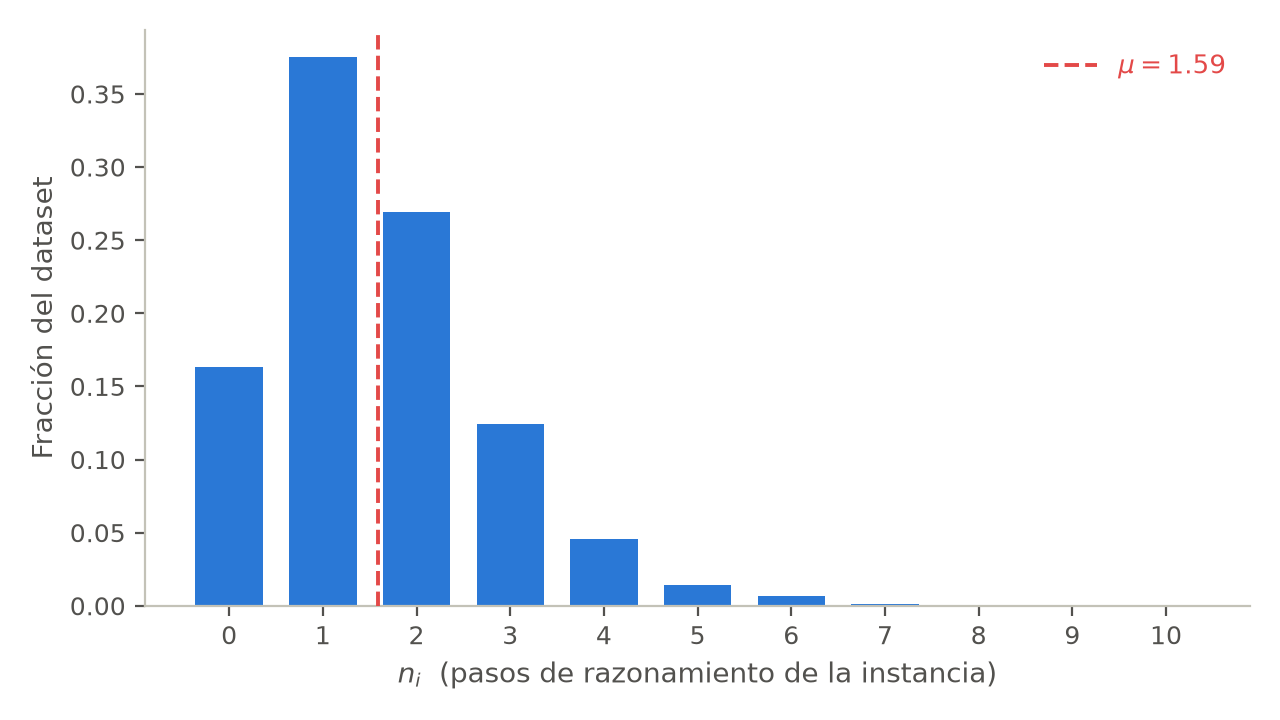
\includegraphics[width=\columnwidth]{figures/step_distribution.png}
  \caption{Distribución del número de pasos de razonamiento anotados $n_i$ en GSM8k-Aug (media $\mu = 1.59$; más de la mitad de los ejemplos con $n_i \le 1$).}
  \label{fig:stepdist}
\end{figure}

\section{Anticipar el presupuesto: predicción \textit{upfront} desde la consigna}
\label{sec:modA}

Antes de construir un mecanismo adaptativo conviene verificar que hay algo que adaptar. Este primer estudio ataca el eje $K$ de la forma más directa: un \emph{barrido oráculo} que mide cuánto presupuesto necesita realmente cada instancia, y un clasificador auxiliar que intenta predecirlo de antemano a partir de la consigna, siguiendo el pipeline \emph{consigna $\rightarrow$ clasificador $\rightarrow$ $\hat{k}$ $\rightarrow$ el modelo razona con $\hat{k}$ pasos}. Todo el estudio se evalúa sobre ejemplos de entrenamiento de GSM8k con una partición de validación interna, no sobre el test held-out del \textit{halting} adaptativo (Sección~\ref{sec:modB}).

\subsection{Barrido oráculo: la premisa se confirma}
\label{sec:ksweep}

Ejecutamos CODI repetidamente sobre los mismos ejemplos variando el número de pasos latentes $k \in \{1,\dots,8\}$, y definimos para cada instancia $k^*$ como el \emph{menor} $k$ que alcanza su mejor puntaje (el presupuesto mínimo suficiente). Sobre $n{=}7473$ ejemplos de entrenamiento de GSM8k, la Tabla~\ref{tab:ksweep} muestra dos hechos. Primero, el presupuesto \textbf{importa}: la accuracy agregada sube $23$ puntos entre $k{=}1$ y $k{\approx}5$--$6$ y luego satura (en $97.4\%$ de los ejemplos la salida cambia al variar $k$). Segundo, el presupuesto óptimo \textbf{varía por instancia} y con fuerte desbalance: el $66\%$ de los ejemplos alcanza su mejor respuesta ya con $k{=}1$, mientras una cola larga necesita $2$ a $8$ pasos. Existe, entonces, la estructura que un mecanismo adaptativo puede explotar: a la mayoría de las instancias les sobra presupuesto y una minoría lo necesita todo.

\begin{table}[t]
  \centering
  \small
  \setlength{\tabcolsep}{4.2pt}
  \begin{tabular}{lcccccccc}
    \toprule
    $k$ & 1 & 2 & 3 & 4 & 5 & 6 & 7 & 8 \\
    \midrule
    Accuracy & .41 & .43 & .48 & .58 & .64 & \textbf{.64} & .64 & .63 \\
    $k^*$ (\%) & \textbf{66.1} & 16.6 & 5.3 & 6.0 & 4.3 & 1.0 & 0.4 & 0.3 \\
    \bottomrule
  \end{tabular}
  \caption{Barrido oráculo sobre CODI ($n{=}7473$ ejemplos de entrenamiento de GSM8k, $k_{\max}{=}8$). Fila superior: accuracy agregada forzando $k$ pasos para todas las instancias. Fila inferior: distribución del presupuesto mínimo óptimo $k^*$ por instancia. La accuracy satura en $k{\approx}5$--$6$ y el $k^*$ está fuertemente desbalanceado hacia $k{=}1$.}
  \label{tab:ksweep}
\end{table}

\subsection{El clasificador \textit{upfront}: un resultado negativo}
\label{sec:clasificador}

La realización más simple de la adaptividad usa esas etiquetas $k^*$ para entrenar un clasificador que prediga el presupuesto \emph{antes} de razonar. Nuestra primera versión, deliberadamente simple, clasifica $k^* \in \{1,\dots,8\}$ sobre embeddings de oración congelados (all-MiniLM-L6-v2, 384 dimensiones; \citealp{reimers2019sbert}), con partición estratificada $5978/1495$. La Tabla~\ref{tab:clasificador} resume la validación interna: el \textit{random forest} balanceado \textbf{colapsa exactamente al baseline de mayoría} (predice $k{=}1$ para los $1495$ ejemplos), y la regresión logística balanceada reparte predicciones pero sólo gana $+0.012$ de F1-macro a costa de hundir la accuracy a $0.21$: dispersa, no discrimina.

\begin{table}[t]
  \centering
  \small
  \begin{tabular}{lcc}
    \toprule
    \textbf{Modelo} & \textbf{Accuracy} & \textbf{F1-macro} \\
    \midrule
    Mayoría (siempre $k{=}1$) & 0.661 & 0.099 \\
    Reg.\ logística (balanceada) & 0.210 & 0.111 \\
    Random forest (balanceado) & 0.661 & 0.099 \\
    \bottomrule
  \end{tabular}
  \caption{Clasificador \textit{upfront} de $k^*$ sobre embeddings congelados (validación interna, $n{=}1495$). Ningún modelo supera a la clase mayoritaria: la representación de la consigna no lleva señal de $k^*$ utilizable por encima de la tasa base.}
  \label{tab:clasificador}
\end{table}

\subsection{De predecir a decidir sobre la marcha}
\label{sec:pivot}

El resultado negativo es informativo porque señala limitaciones estructurales del enfoque \textit{upfront}, no sólo de su primera implementación. (i) El clasificador debe inferir la dificultad mirando \emph{sólo la consigna}, antes de que el modelo principal empiece a razonar y sin acceso a sus estados ocultos; la señal que necesita puede simplemente no estar en una representación estática del texto. (ii) Construir las etiquetas cuesta $k_{\max}$ pasadas del modelo por instancia, y $k^*$ hereda el desbalance y el ruido de la métrica con que se puntúa. (iii) La decisión se toma una sola vez: si $\hat{k}$ queda corto, el sistema no puede corregirse sobre la marcha. El \textit{halting} adaptativo (Sección~\ref{sec:modB}) disuelve los tres problemas: decide \emph{durante} el razonamiento observando los propios estados latentes, no necesita etiquetas $k^*$, y se optimiza directamente por la señal de tarea.

\section{Decidir sobre la marcha: \textit{halting} probabilístico tipo PonderNet}
\label{sec:modB}

En lugar de fijar $K$ o de predecirlo antes de razonar (la predicción \textit{upfront}, Sección~\ref{sec:modA}), decidimos el punto de detención \emph{durante} el razonamiento: injertamos el \textit{halting} probabilístico de PonderNet sobre el bucle de pensamientos continuos de $K$ fijo (Ecuación~\ref{eq:latentloop}), de modo que el modelo aprende cuántos pasos latentes usar por instancia observando sus propios estados. La Figura~\ref{fig:posterfrontier} adelanta el resultado central: el modelo adaptativo iguala la accuracy del baseline de $K$ fijo gastando cerca de la mitad del cómputo.

\begin{figure}[!hb]
  \centering
  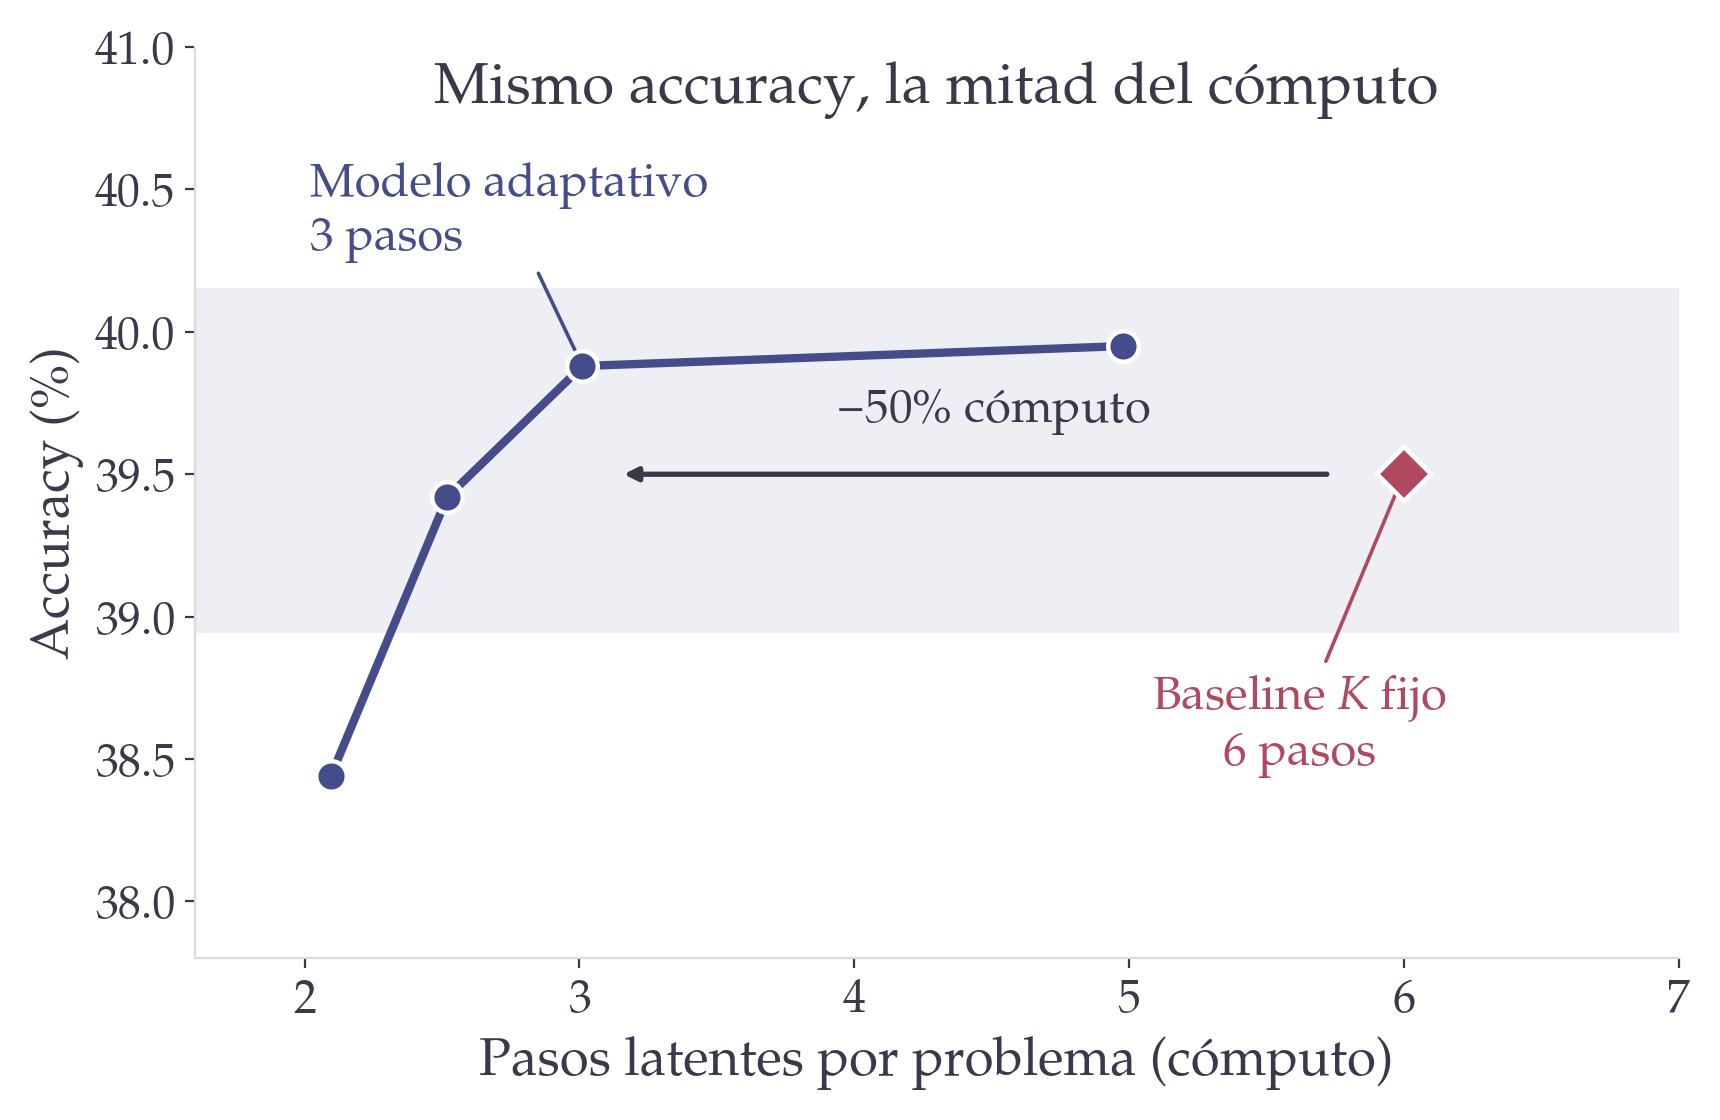
\includegraphics[width=\columnwidth]{figures/poster_frontier-ap.png}
  \caption{Resultado central del \textit{halting} adaptativo. El modelo adaptativo (M2) alcanza la accuracy del baseline de $K$ fijo ($\approx 39.5\%$) con $\sim 3$ pasos latentes por problema, la mitad de los $6$ pasos del baseline. Cada punto azul es un threshold de detención distinto del mismo modelo; el rombo es el baseline. Test held-out ($n{=}1319$).}
  \label{fig:posterfrontier}
\end{figure}

\subsection{Halting adaptativo}
\label{sec:halting}

Añadimos una única cabeza lineal de \textit{halting}, $\texttt{halt\_head}: \mathbb{R}^d \rightarrow \mathbb{R}$, cuyo sesgo se inicializa en $-2.0$ (de modo que la probabilidad de detención inicial es $\sigma(-2)\approx 0.12$ y el modelo usa muchos pasos al comienzo del entrenamiento). En cada paso latente $k$ define una \emph{probabilidad de detención condicional}
\begin{equation}
  \lambda_k = \sigma\!\left(\texttt{halt\_head}(h_k)\right),
\end{equation}
la probabilidad de detenerse en el paso $k$ dado que no se detuvo antes. A diferencia del $K$ fijo, decodificamos una respuesta candidata tras \textbf{cada} prefijo $k = 1,\dots,K$, lo que permite construir la \emph{distribución de terminación} geométrica de PonderNet:
\begin{equation}
  p_k = \Bigg(\prod_{j<k}\big(1 - \lambda_j\big)\Bigg)\,\lambda_k .
  \label{eq:halting}
\end{equation}
Para que la distribución sume 1 sin perder masa, imponemos una \emph{frontera absorbente} en $K$ (equivalente a forzar $\lambda_K \rightarrow 1$): la última entrada recibe toda la masa restante $p_K = \prod_{j<K}(1-\lambda_j)$, y luego se renormaliza.

\subsection{Objetivo de entrenamiento}
\label{sec:loss}

El objetivo combina tres linajes. De PonderNet, la \emph{pérdida esperada de respuesta} y la regularización KL; de SIM-CoT, la supervisión por paso; de CODI, la destilación:
\begin{equation}
  \mathcal{L} = \mathcal{L}_{\text{ponder}}
  + \beta_{\text{step}}\,\mathcal{L}_{\text{step}}
  + \gamma\,\mathrm{KL}_{\text{geom}}
  + \mathcal{L}_{\text{distill}}
  + \mathcal{L}_{\text{ref}} .
  \label{eq:loss}
\end{equation}
El término principal pondera la entropía cruzada de respuesta de cada prefijo por su probabilidad de detención,
\begin{equation}
  \mathcal{L}_{\text{ponder}}
  = \sum_{k=1}^{K} p_k \, \mathcal{L}_{\text{ans}}^{(k)} ,
  \label{eq:lponder}
\end{equation}
de modo que el modelo aprende a hacer buenas las respuestas de los prefijos a los que asigna masa. $\mathcal{L}_{\text{step}}$ es la reconstrucción del decoder auxiliar de SIM-CoT (con $\beta_{\text{step}}=1.0$; el decoder se descarta en inferencia). $\mathrm{KL}_{\text{geom}}$ es la divergencia KL de la distribución de terminación $p_k$ hacia un \emph{prior geométrico truncado} $q$ de media \texttt{geom\_mean}; con $g = 1/\texttt{geom\_mean}$, $q_k \propto (1-g)^{k}\,g$ con la misma frontera absorbente en $K$. Los términos $\mathcal{L}_{\text{distill}}$ (alineación SmoothL1 de estados ocultos maestro--estudiante) y $\mathcal{L}_{\text{ref}}$ (entropía cruzada de la tarea maestra) provienen de CODI. Por defecto $\gamma=0.01$ y $\texttt{geom\_mean}=3.0$. El peso $\gamma$ es la palanca causal que regula cuánto se acorta el cómputo: sube la presión hacia detenerse antes.

\subsection{Prior geométrico por instancia}
\label{sec:prior}

Un prior geométrico \emph{global} pide el mismo presupuesto esperado a todos los problemas. Lo reemplazamos por un prior \textbf{por instancia} que ancla el presupuesto al número de operaciones $n_i$ del problema mediante un mapeo afín:
\begin{equation}
  \texttt{geom\_mean}_i = \mathrm{clamp}\big(\alpha\, n_i + \beta,\; \beta,\; K_{\max}\big).
  \label{eq:adaptiveprior}
\end{equation}
La forma afín (y no la identidad $\texttt{geom\_mean}_i = n_i$) es necesaria por la asimetría de la distribución de $n_i$ en GSM8k-Aug (Figura~\ref{fig:stepdist}): más de la mitad de los ejemplos tienen $n_i \le 1$, que bajo la identidad caerían en un prior degenerado de masa puntual ($g=1$), cuyo KL domina la pérdida de tarea. El desplazamiento $\beta$ levanta a todos los ejemplos de ese piso.

\subsection{Inferencia}
\label{sec:inferencia}

En inferencia acumulamos masa de detención paso a paso y cortamos el bucle latente en cuanto la masa acumulada cruza un threshold (por defecto $0.5$); $K_{\max} = \texttt{max\_latent\_steps}$ es un tope duro. La respuesta se decodifica desde el prefijo en el que la instancia se detuvo. Un detalle de fidelidad: como los pasos latentes se comparten dentro de un batch pero cada ejemplo se detiene en un paso distinto, una evaluación fiel requiere \texttt{batch\_size}$=1$ (o cortar la KV-cache fila por fila en el paso de detención de cada ejemplo); de lo contrario un ejemplo que para temprano se decodificaría desde un prefijo más largo del que su cuenta de pasos reporta. Todos los números de este trabajo usan la variante fiel. El checkpoint (época) y el threshold de detención se eligieron en un set de validación separado de $500$ ejemplos, nunca sobre el test held-out en el que se reportan las cifras de esta sección.

\subsection{La frontera accuracy--cómputo}
\label{sec:frontera}

El resultado central de este estudio es que el modelo adaptativo traza una \textbf{frontera} accuracy--pasos que el $K$ fijo no puede: variando $\gamma$ (que hace ``morder'' al prior geométrico) y la forma del prior por instancia, movemos monótonamente el punto de operación. La Tabla~\ref{tab:frontera} compara, por threshold de detención, tres puntos de operación que difieren únicamente en la fuerza $\gamma$ del regularizador KL y la pendiente $\alpha$ del prior por instancia: \textbf{M0} (el prior débil de referencia), \textbf{M1} (que endurece $\gamma$) y \textbf{M2} (que además baja $\alpha$ para recortar la cola de presupuesto en los problemas difíciles). Los valores exactos de cada configuración están en la tabla.

\begin{table}[t]
  \centering
  \small
  \begin{tabular}{lccc}
    \toprule
    \textbf{Threshold} & \textbf{M0} & \textbf{M1} & \textbf{M2} \\
                    & $\alpha1.0,\gamma.05$ & $\alpha1.0,\gamma.10$ & $\alpha0.6,\gamma.10$ \\
    \midrule
    0.3 & 39.1 @ 3.34 & 39.1 @ 2.60 & 38.4 @ \textbf{2.10} \\
    0.4 & 39.6 @ 3.86 & 39.4 @ 3.16 & 39.4 @ \textbf{2.52} \\
    0.5 & 40.0 @ 4.46 & 39.4 @ 3.73 & \textbf{39.9 @ 3.01} \\
    0.8 & 40.2 @ 6.97 & 39.7 @ 6.39 & 40.0 @ 4.98 \\
    \bottomrule
  \end{tabular}
  \caption{Frontera accuracy--cómputo. Cada celda es \emph{accuracy (\%) @ pasos latentes promedio}, en el conjunto de test held-out ($n=1319$), \textit{greedy}, \texttt{batch\_size}$=1$. La accuracy queda a la par entre las tres configuraciones ($\sim 39$--$40\%$); subir $\gamma$ (M1) y bajar $\alpha$ (M2) recortan los pasos a accuracy de paridad. (M0/M1/M2 son el mismo modelo a tres configuraciones de $\gamma$ y forma del prior.)}
  \label{tab:frontera}
\end{table}

\begin{figure}[t]
  \centering
  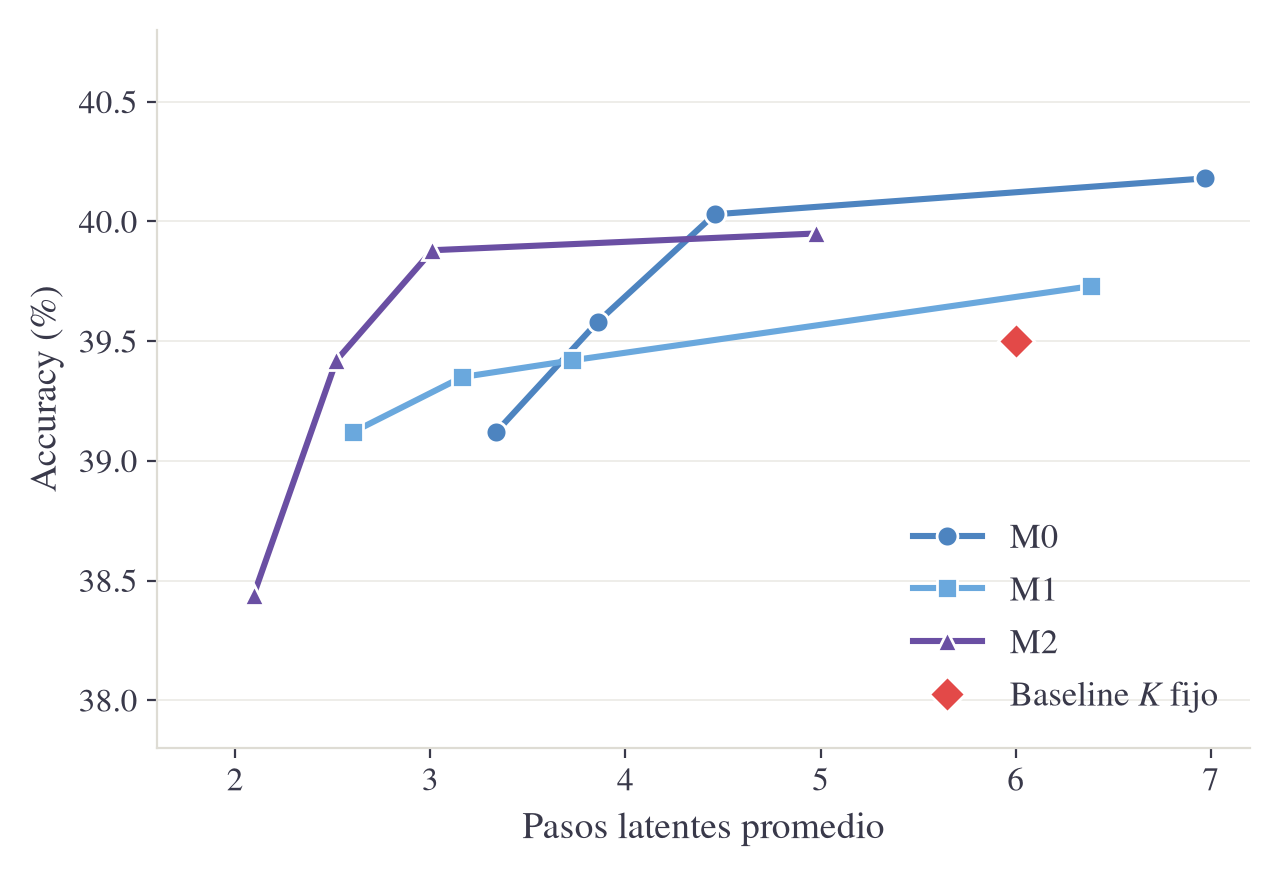
\includegraphics[width=\columnwidth]{figures/frontier_test-ap.png}
  \caption{Frontera accuracy--cómputo. Subir $\gamma$ desplaza la frontera hacia la izquierda (menos pasos a igual accuracy); bajar la pendiente $\alpha$ del prior por instancia recorta aún más la cola de presupuesto. M2 alcanza $39.9\%$ con $3.01$ pasos, un $33\%$ menos que M0 a igual threshold ($40.0\%$ a $4.46$ pasos) y la mitad que el baseline de $K$ fijo ($6$ pasos).}
  \label{fig:frontera}
\end{figure}

En test la accuracy es esencialmente plana ($\sim 39$--$40\%$) entre configuraciones y thresholds, de modo que la elección del punto de operación es de \emph{presupuesto de cómputo}. El punto de mínimo cómputo a paridad es \textbf{M2} a threshold $0.5$: $\mathbf{39.9\%}$ con $\mathbf{3.01}$ pasos, igualando al baseline de $K$ fijo ($39.5\%$) con la \textbf{mitad} de los pasos, y $-33\%$ pasos frente a M0 al mismo threshold (a $-0.1$ pp). Bajar el threshold a $0.4$/$0.3$ comprime aún más el cómputo (M2: $2.52$/$2.10$ pasos) con caídas de accuracy pequeñas. Un $\gamma$ demasiado bajo ($0.05$, M0) hace que el prior no muerda; subirlo a $0.10$ (M1/M2) desplaza toda la frontera hacia la izquierda. La Figura~\ref{fig:frontera} lo visualiza. La paridad de accuracy además se sostiene \emph{bin a bin} de dificultad (Figura~\ref{fig:accbydiff}): el recorte de cómputo no se paga en ningún régimen, ni en los problemas fáciles ni en los difíciles.

\begin{figure}[b]
  \centering
  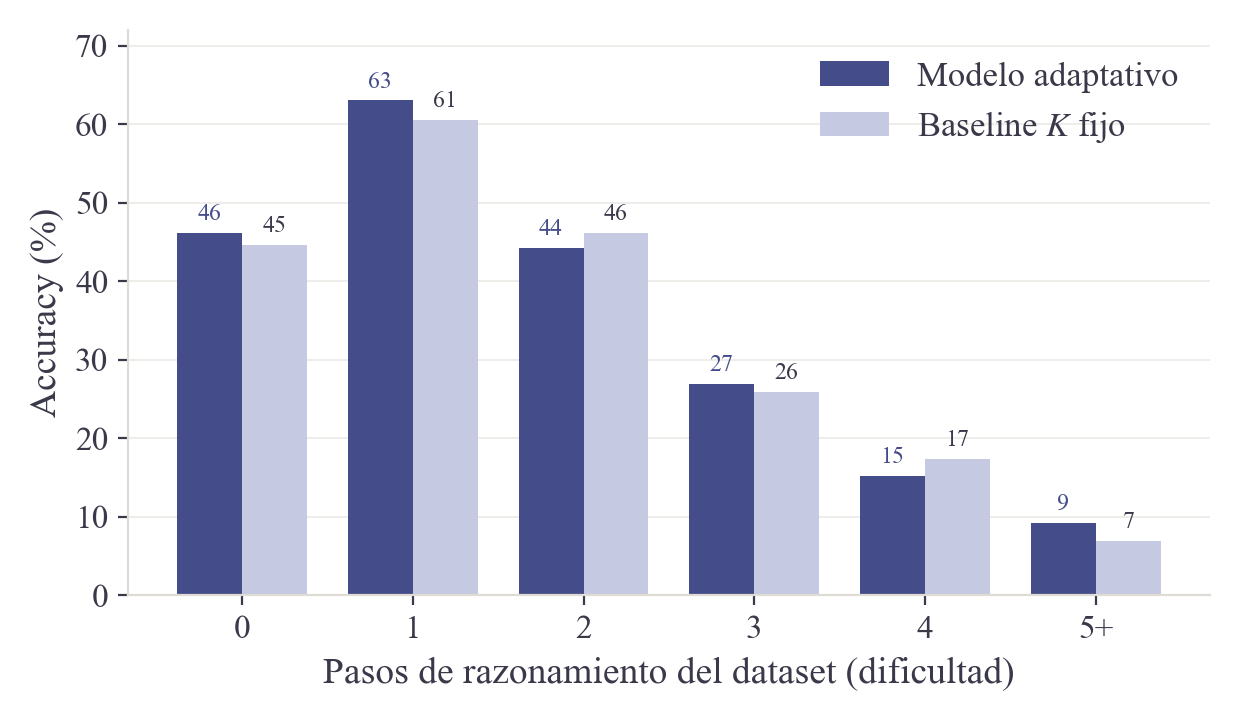
\includegraphics[width=\columnwidth]{figures/accuracy_by_difficulty-ap.png}
  \caption{Accuracy por nivel de dificultad (pasos de razonamiento anotados del dataset) del modelo adaptativo (M2, threshold $0.5$) frente al baseline de $K$ fijo, en test held-out. La paridad se mantiene bin a bin: la ventaja del modelo adaptativo es de cómputo, no de accuracy, en toda la escala de dificultad.}
  \label{fig:accbydiff}
\end{figure}

\subsection{Seguimiento de dificultad}
\label{sec:dificultad}

Un modelo verdaderamente adaptativo debería gastar más pasos en los problemas más difíciles. Medimos esto con la correlación de Spearman entre el número de operaciones $n_{\text{expr}}$ y los pasos usados. En el conjunto de test held-out, el punto de mínimo cómputo (M2, threshold $0.5$) alcanza $\mathbf{+0.626}$ (M0 y M1 llegan más alto todavía: $+0.677$ y $+0.675$ respectivamente), una correlación fuerte que confirma que el afinado de scope completo con prior por instancia y $K_{\max}=12$ asigna cómputo por dificultad. La Figura~\ref{fig:jointmatrix} lo muestra directamente: la distribución conjunta de dificultad y pasos usados concentra su masa a lo largo de la diagonal.

\begin{figure}[t]
  \centering
  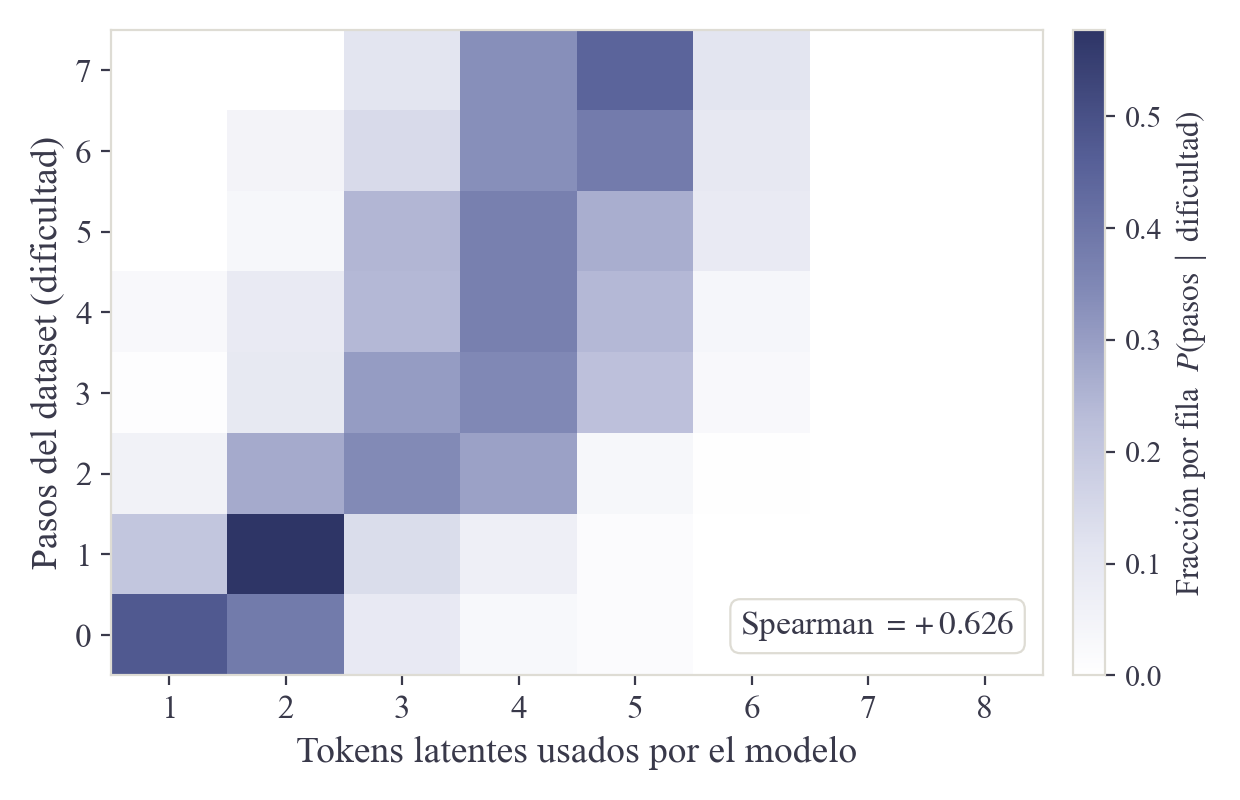
\includegraphics[width=\columnwidth]{figures/joint_matrix-ap.png}
  \caption{Distribución conjunta de la dificultad del problema (pasos anotados del dataset, filas) y los pasos latentes que el modelo efectivamente usa (columnas), normalizada por fila. La masa se corre hacia la derecha al descender por las filas: el modelo gasta más pasos en los problemas más difíciles (Spearman $+0.626$). M2, threshold $0.5$, test held-out.}
  \label{fig:jointmatrix}
\end{figure}

El efecto es interpretable a nivel de grupo de dificultad (Figura~\ref{fig:stepsaccbydiff}): en esa configuración (M2, test, threshold $0.5$), los pasos promedio escalan de $1.72$ (problemas de $0$ operaciones) a $2.11$, $2.99$, $3.77$, $3.81$ y $\sim 4.1$--$4.6$ (problemas de $5$ o más operaciones). Los problemas fáciles se detienen alrededor de dos pasos y los difíciles alrededor de cuatro y medio: el modelo asigna cómputo por dificultad, no por un presupuesto uniforme.

\begin{figure}[b]
  \centering
  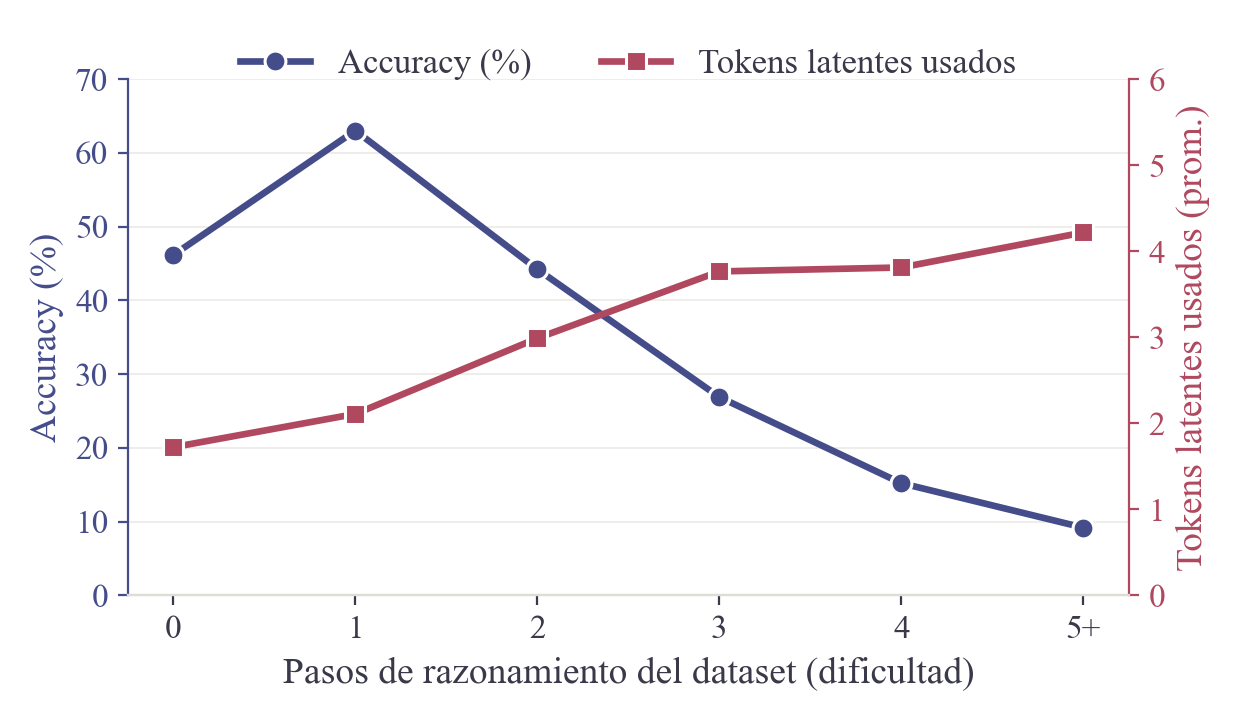
\includegraphics[width=\columnwidth]{figures/steps_accuracy_by_difficulty-ap.png}
  \caption{Pasos latentes promedio usados (rojo, eje derecho) y accuracy (azul, eje izquierdo) por nivel de dificultad, para el modelo adaptativo (M2, threshold $0.5$) en test held-out. Los pasos usados crecen monótonamente con la dificultad mientras la accuracy cae: el cómputo se asigna donde el problema lo exige.}
  \label{fig:stepsaccbydiff}
\end{figure}

\subsection{Hacia una comparación justa desde cero}
\label{sec:fromscratch}

Los experimentos anteriores parten de un warm-start del checkpoint CODI completo (backbone, LoRA, proyección y decoder, producto de un entrenamiento CODI que no realizamos), y luego afinan sólo cinco épocas. Un revisor puede preguntar, con razón, si el $\approx 40\%$ proviene del \emph{método} adaptativo o del checkpoint heredado. Para aislarlo, replicamos \textbf{M2} (la configuración de mínimo cómputo) desde un GPT-2 \emph{vanilla}: se entrena también el decoder auxiliar (un nuevo \textit{scope} \texttt{full\_dec}), sobre el GSM8k-Aug completo, $40$ épocas. Registramos una corrección de receta necesaria: la tasa $3\times10^{-3}$ del trabajo original diverge en \texttt{bf16} (la norma del gradiente explota y aparece \texttt{NaN}); $1\times10^{-3}$ con \textit{warmup} $0.05$ es estable. Al momento de la entrega de este trabajo, el modelo desde cero \textbf{todavía se está entrenando} (transferido a una GPU A100 por el costo del bucle secuencial de $K=12$). El objetivo es reportar tres puntos comparables (baseline de $K$ fijo, adaptativo con warm-start, y adaptativo desde cero) de modo que la brecha cuantifique el aporte del warm-start frente al del método.

\section{El segundo eje del presupuesto: vectores por paso}
\label{sec:modC}

El presupuesto latente tiene un segundo eje: cuántos vectores $c$ representan cada paso de razonamiento. Coconut usa $c{=}2$ fijo; el checkpoint CODI del que partimos, $c{=}1$. Este tercer estudio hace ese número variable por paso: cada paso se construye como un bloque de hasta $M$ sub-vectores generados uno a uno, el decoder auxiliar de SIM-CoT reconstruye el texto del paso desde el bloque acumulado, y un MLP liviano \emph{destila} esa pérdida de reconstrucción $\mathcal{L}_{\text{step}}$ desde el estado oculto ($\hat{\mathcal{L}} = \mathrm{MLP}(h)$, pérdida SmoothL1). A diferencia del decoder, el MLP sobrevive a la inferencia: tras cada sub-vector se evalúa $\hat{\mathcal{L}}$ y, cuando converge ($|\hat{\mathcal{L}}_j - \hat{\mathcal{L}}_{j-1}| < \varepsilon$), el paso se considera semánticamente maduro y el modelo avanza al siguiente. Una \textit{ponder penalty} opcional penaliza sub-vectores extra cuando el paso ya parece maduro.

\paragraph{El mecanismo funciona; el eje no tiene margen.} Entrenado con warm-start sobre la segmentación atómica de GSM8k-Aug (una operación aritmética por paso) y evaluado sobre el conjunto de test completo ($n{=}1319$, \texttt{batch\_size}$=1$), el \textit{halting} adaptativo recorta entre un $16\%$ y un $33\%$ de los vectores latentes sin costo de accuracy ($\approx 39.5$--$39.9\%$, competitivo con el baseline). Pero a presupuesto igualado \textbf{no supera ni al \textit{halting} aleatorio ni a un $c$ fijo}: la curva de accuracy contra $c$ fijo (Tabla~\ref{tab:opcionb}, primera fila) sube $+11.9$ puntos de $c{=}1$ a $c{=}2$ y sólo $+0.5$ de $c{=}2$ a $c{=}3$. Satura duro en $c{=}2$, de manera casi uniforme entre instancias: el MLP ni siquiera asigna más vectores a los problemas que el modelo falla (correctos $10.28$ contra incorrectos $10.01$ vectores en promedio). El eje $c$ importa, pero su \emph{varianza por instancia} es casi nula en esta tarea: el óptimo simple es $c{=}2$ fijo, y no hay adaptividad inteligente que explotar.

\begin{table}[t]
  \centering
  \small
  \begin{tabular}{lcccc}
    \toprule
    \textbf{Init $\times$ granularidad} & $c{=}1$ & $c{=}2$ & $c{=}3$ & $\Delta_{2\rightarrow3}$ \\
    \midrule
    warm $+$ atómica & 27.5 & 39.4 & 39.9 & $+0.5$ \\
    warm $+$ gruesa & 25.5 & 36.6 & \textbf{40.3} & $+3.7$ \\
    \textit{cold} $+$ gruesa & 5.3 & 5.5 & 5.5 & n/d \\
    \bottomrule
  \end{tabular}
  \caption{Accuracy (\%) con $c$ fijo forzado, por inicialización y granularidad de segmentación (test de GSM8k, $n{=}1319$). Con pasos atómicos la curva satura en $c{=}2$; con pasos gruesos (2--3 operaciones, densidad variable) el tercer vector vuelve a aportar. Desde cero el modelo colapsa: los latentes quedan inertes.}
  \label{tab:opcionb}
\end{table}

\paragraph{El negativo es de la granularidad, no del mecanismo.} Dos controles acotan la conclusión. Primero, reentrenar \emph{desde cero} (GPT-2 vanilla, decoder fresco) colapsa a casi azar ($\approx 5.5\%$ para todo $c$): el modelo aprende el formato de la respuesta pero los latentes quedan inertes (decodificar tras cada prefijo da una curva plana), es decir, el razonamiento latente no arranca de cero bajo este objetivo y el warm-start no era un sesgo sino una pieza estructural. Segundo (y más interesante), re-segmentar los pasos de forma \emph{gruesa} (agrupando 2--3 operaciones por paso, con densidad variable) sobre el modelo warm revive la señal: el salto $c{=}2 \rightarrow c{=}3$ pasa de $+0.5$ a $+3.7$ puntos (Tabla~\ref{tab:opcionb}), y el \textit{halting} adaptativo pasa a superar al \textit{halting} aleatorio por $+3.6$ puntos ($\approx 2.7\sigma$; $38.8\%$ con $7.2$ vectores contra $35.2\%$ con $6.1$), algo que en el régimen atómico no ocurría, aunque la ganancia sobre asignar a todos el mismo presupuesto es modesta ($+0.6$ a $+1.0$). La lectura conjunta: en GSM8k-Aug cada paso atómico es una operación trivial que dos vectores saturan; la varianza de la tarea vive en el \emph{número} de pasos, no en su complejidad interna. Esto acota el espacio de diseño y refuerza la elección del eje $K$ como el que tiene dinámica real.

\section{Discusión}

Interpretamos el \textit{halting} aprendido como un mecanismo de \emph{early-exit} que evita el régimen de alto-$K$ propenso al colapso. SIM-CoT \citep{wei2025simcot} documenta que los latentes tardíos se homogeneizan y se limitan a ``repetir'' la predicción final una vez alcanzada la respuesta; detenerse cuando la respuesta ya está codificada preserva la diversidad entre latentes y actúa como regularizador del número de pasos, sin tratarlo como un hiperparámetro a ajustar. Que la accuracy quede dentro del ruido es coherente con esta lectura: el método no busca resolver problemas que el $K$ fijo no resuelve, sino resolver los mismos gastando cómputo proporcional a la dificultad. La frontera de la Figura~\ref{fig:frontera} es la formulación operativa de esa idea.

Leídos en conjunto, los tres estudios delimitan dónde aparece la adaptividad en esta familia: el barrido oráculo (Sección~\ref{sec:modA}) muestra que el presupuesto óptimo varía por instancia; que la predicción \textit{upfront} no supere la tasa base muestra que esa variación no es legible desde una representación estática de la consigna; y la exploración del eje $c$ (Sección~\ref{sec:modC}) muestra que tampoco vive en la densidad interna de cada paso. Queda el \emph{número} de pasos, decidido durante el razonamiento (Sección~\ref{sec:modB}), como el eje con dinámica explotable.

\section*{Limitaciones}

Varias salvedades acotan nuestras conclusiones. Primero, aun con $1319$ ejemplos de test, diferencias de accuracy de fracciones de punto están dentro del ruido de muestreo; nuestras afirmaciones de accuracy son de \emph{paridad}, no de mejora. Segundo y tercero comparten una raíz: nuestro presupuesto de cómputo acotado. Por él evaluamos un único backbone (GPT-2) y una única tarea (GSM8k), de modo que no sabemos cómo escala la adaptividad a modelos mayores u otros dominios de razonamiento; y por esa misma restricción la comparación justa desde cero (Sección~\ref{sec:fromscratch}), cuyo bucle secuencial de $K{=}12$ es particularmente costoso, todavía se está entrenando al momento de la entrega y no tiene número final. Cuarto, como declaramos al presentar cada estudio (Sección~\ref{sec:setup}), la predicción \textit{upfront} se evaluó sobre ejemplos de entrenamiento con validación interna, mientras que el \textit{halting} adaptativo y el eje $c$ comparten el test de GSM8k ($1319$ ejemplos held-out): las cifras de la predicción \textit{upfront} no son directamente comparables con las otras, y la comparación \textit{end-to-end} entre predecir $k$ \textit{upfront} y el \textit{halting} aprendido quedó pendiente. Por último, nuestro criterio de detención en inferencia es un threshold determinista sobre la masa acumulada, que difiere del muestreo Bernoulli de la formulación original de PonderNet \citep{banino2021pondernet}; no comparamos ambos regímenes.

\section{Conclusión}

Estudiamos cómo volver adaptativo por instancia el presupuesto de razonamiento latente, explorando sus dos ejes en tres estudios. La predicción \textit{upfront} confirmó la premisa con un barrido oráculo (el presupuesto óptimo de pasos existe, varía por instancia y satura), pero dejó un resultado negativo informativo: anticipar ese presupuesto desde embeddings congelados de la consigna no supera la tasa base. El \textit{halting} adaptativo, el que sí funciona, decide \emph{durante} el razonamiento: injertamos el \textit{halting} probabilístico de PonderNet sobre la pila CODI/SIM-CoT y, en el conjunto de test held-out, el modelo iguala la accuracy del baseline de $K$ fijo ($\approx 39.5\%$ en GSM8k con GPT-2) recortando cerca de la mitad ($\sim 50\%$) de los pasos latentes, con un fuerte seguimiento de la dificultad (Spearman $+0.626$). El estudio del eje $c$ mostró que ese otro eje, el de vectores por paso, casi no tiene varianza explotable en GSM8k-Aug. El aporte no es una accuracy mayor sino \textbf{adaptividad de cómputo}: la caracterización de la frontera accuracy--pasos que la familia del CoT implícito, atada a un $K$ fijo, nunca reportó.

% Custom bibliography entries only
\bibliography{custom}

\end{document}
